%!TEX root = final_report.tex

\subsection{Unit tests on synthetic datasets}
We tested our implementation on simulated data sets to check its correctness. We generated 4 test sets in the 3-dimensional space and 3 test cases in the 4-dimensional space. Figure \ref{fig: testcases} show a visualization of our 3-dimensional test cases. For simplicity, the range on each axis is set to be $[0, 20]$. In test set 1, there is just a box in the middle of the space. In test set 2, there is one box floating in the middle of the space as well as four smaller boxes on the other side of the space. The smaller boxes, however, should be able to be identified as 1 dense sub-tensor, since the Dcube algorithm is scanning for subsets, rather than continuous ranges, of unique values associated with high density (though definition of density could vary) on each dimension. The four smaller boxes can be expressed the cartesian product of one subset of values along each dimension, therefore they should be identified in the same dense block. In test set 3, we have 3 boxes of various sizes next to each other. A correct implementation should be able to identify the 3 boxes separately. In test set 4, we have  3 boxes alone the spacial diagonal of the space. We expect the algorithm to identify all three boxes easily.

\begin{figure}[h]
\centering 
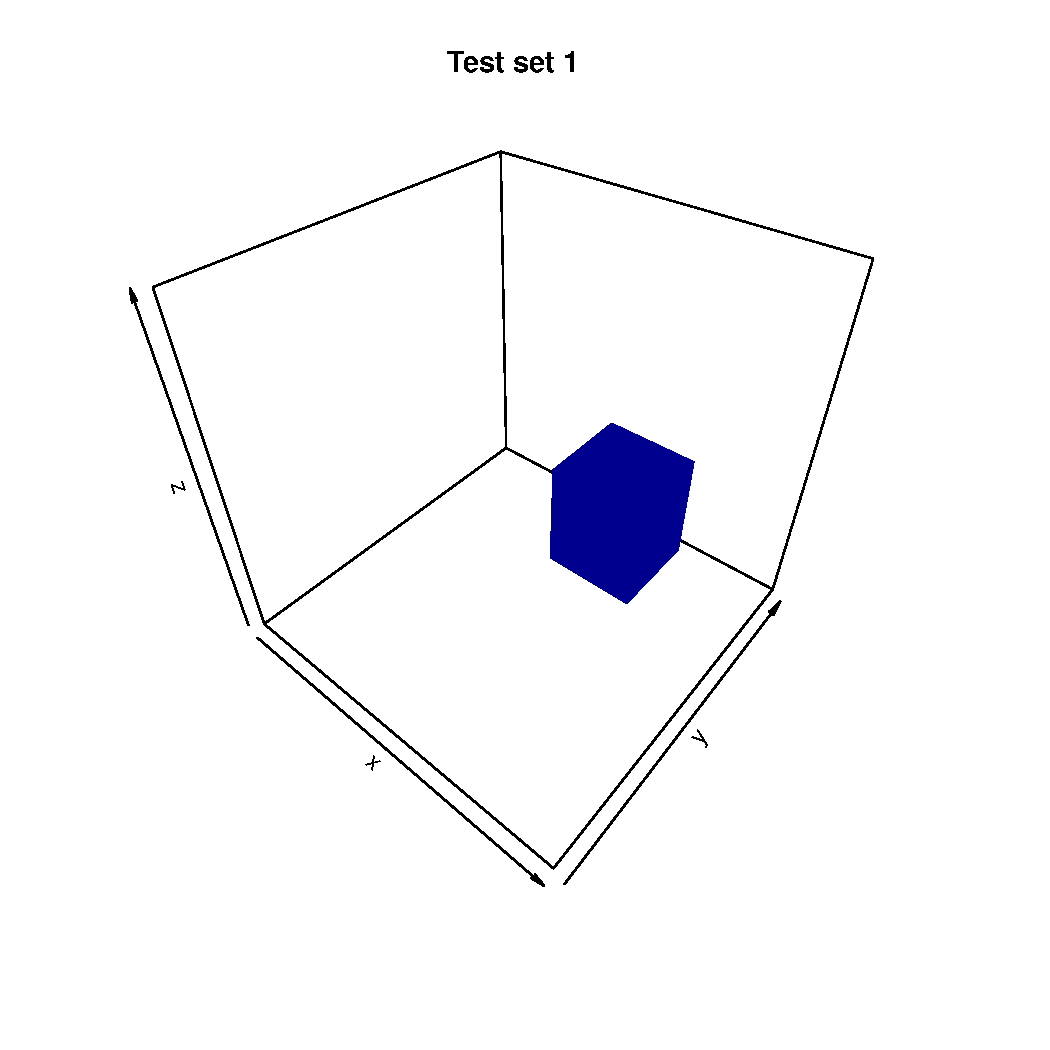
\includegraphics[width=.35\columnwidth]{plots/TS1.pdf} 
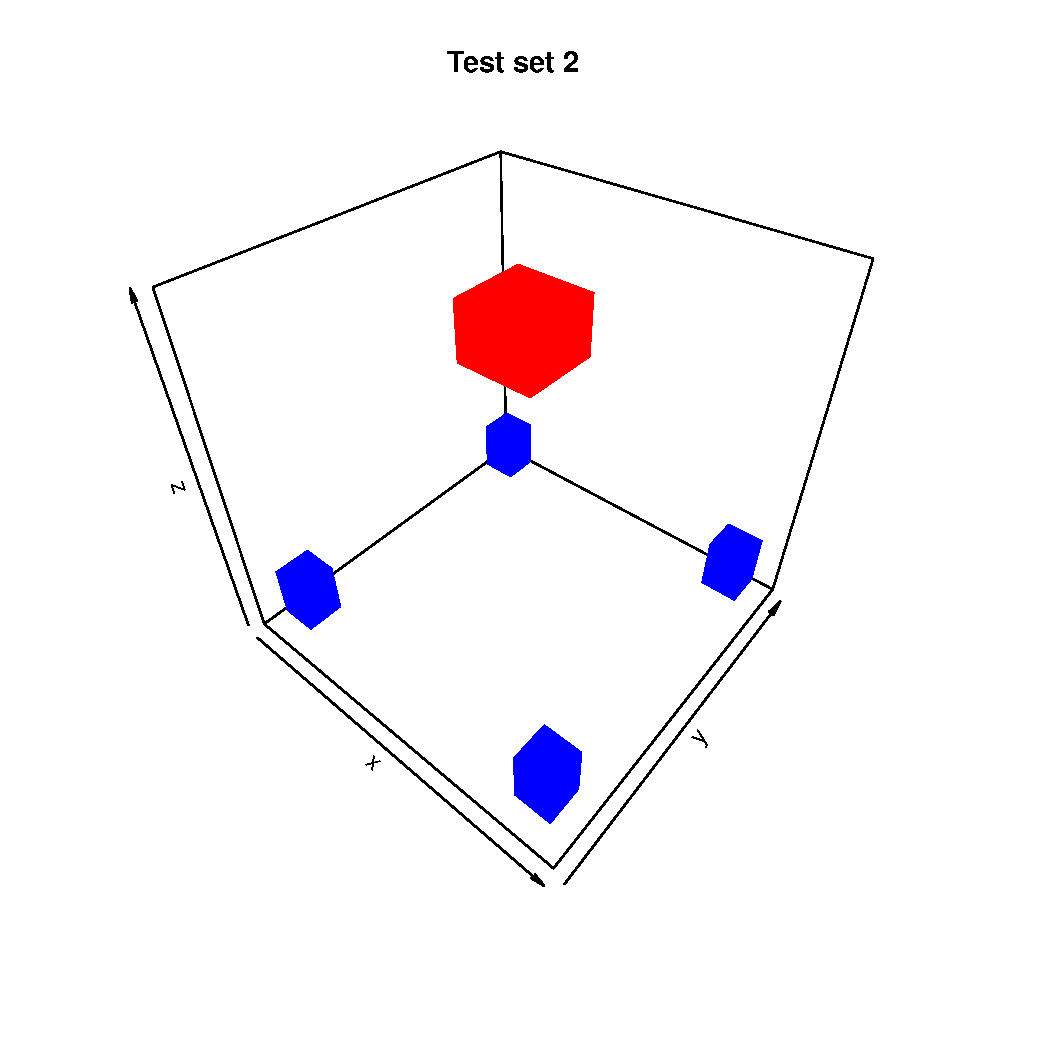
\includegraphics[width=.35\columnwidth]{plots/TS2.pdf} 
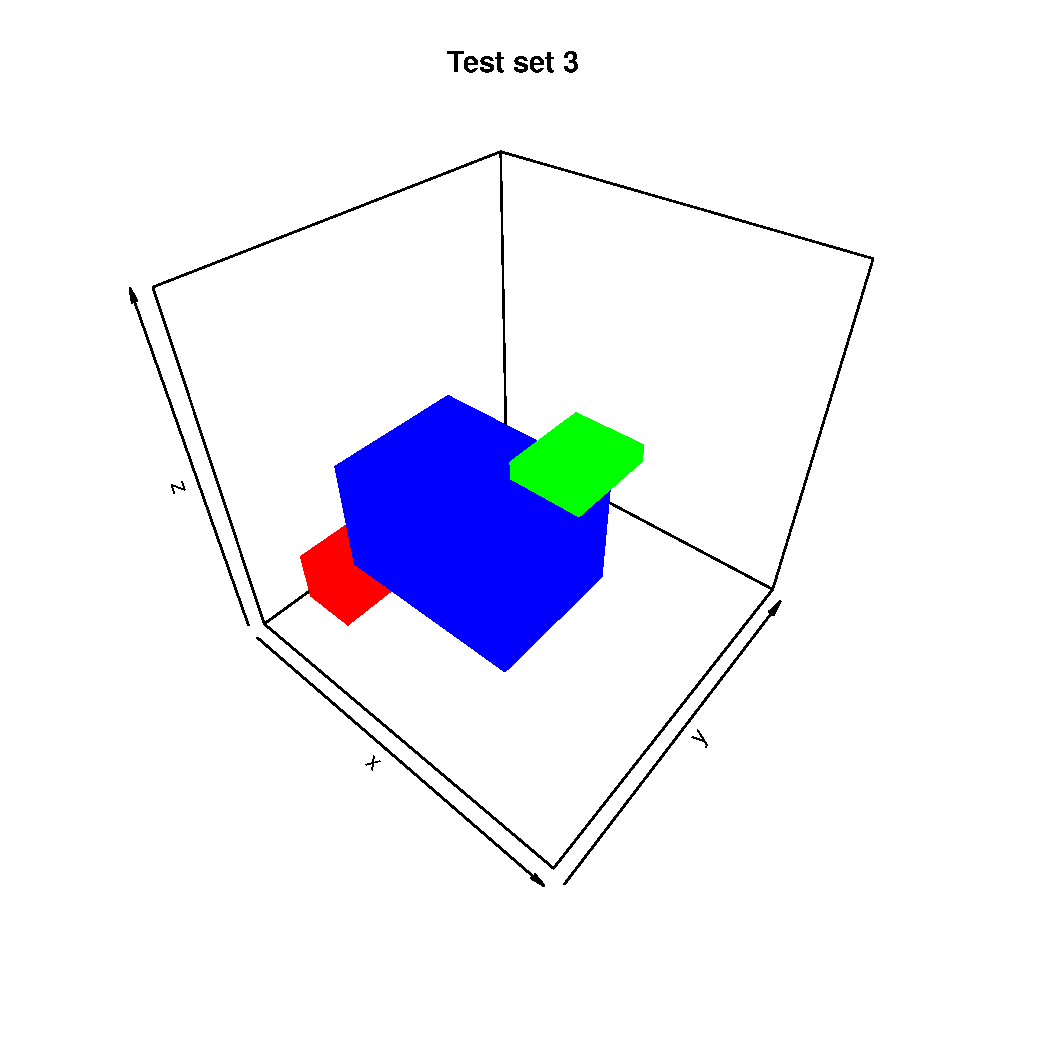
\includegraphics[width=.35\columnwidth]{plots/TS3.pdf} 
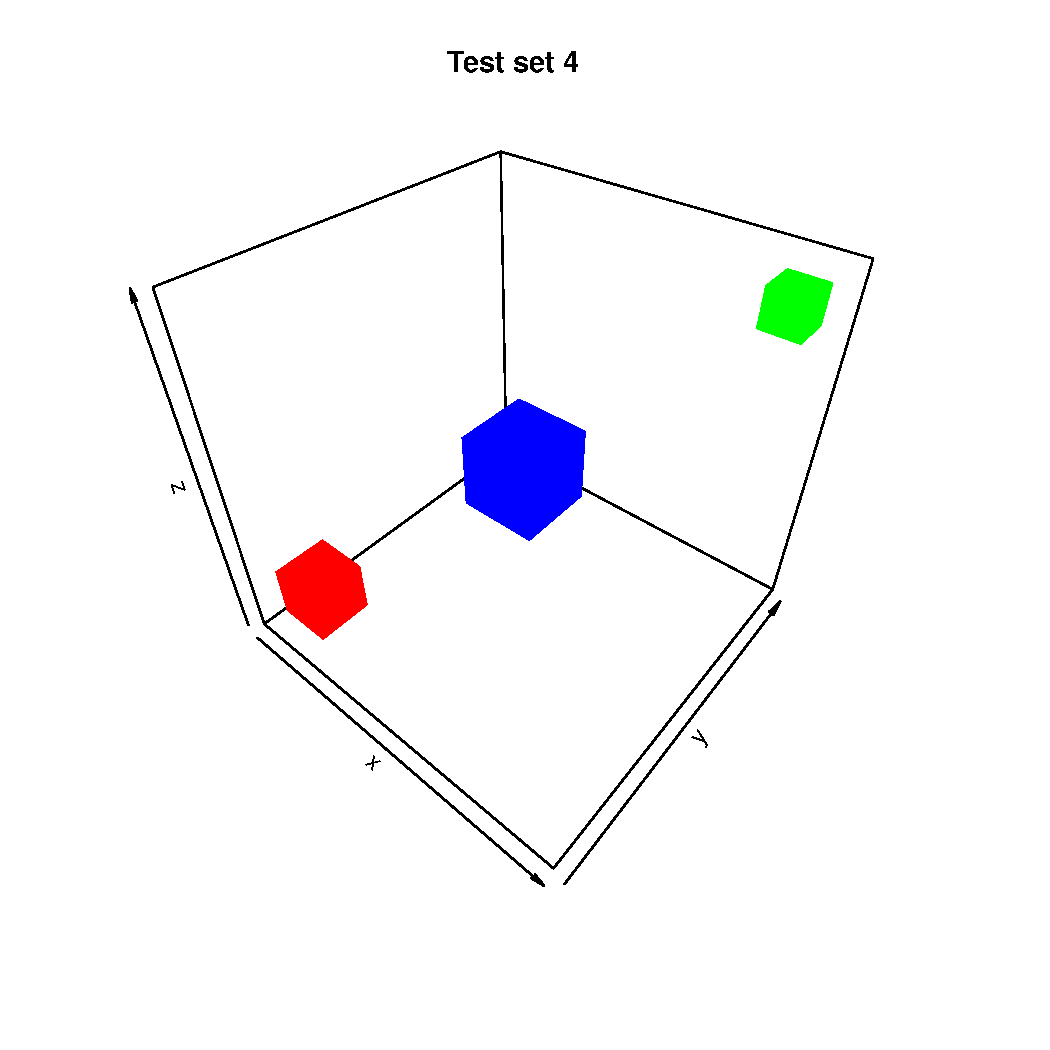
\includegraphics[width=.35\columnwidth]{plots/TS4.pdf} 
\caption{True blocks in test data sets. }
\label{fig: testcases}
\end{figure}

\begin{table}[h]
\centering
\caption{Summary of unit test results in the 3-dimensional space}
\label{table: test3d}
\begin{tabular}{r|r|r|r|r|r|r }
\hline
\multicolumn{1}{c|}{\multirow{2}{*}{\begin{tabular}[c]{@{}c@{}}Dimensionality Selection Policy\\ Density Measure\end{tabular}}} & \multicolumn{3}{c|}{Maximum Density First}                                                  & \multicolumn{3}{c}{Maximum Cardinality First}                                              \\ \cline{2-7} 
\multicolumn{1}{c|}{}                                                                                                           & \multicolumn{1}{c|}{Dataset} & \multicolumn{1}{c|}{Precision} & \multicolumn{1}{c|}{Recall} & \multicolumn{1}{c|}{Dataset} & \multicolumn{1}{c|}{Precision} & \multicolumn{1}{c}{Recall} \\ \hline
\multirow{4}{*}{Arithmatic Average Degree}                                                                                       & Test set 1                   & 1.0                            & 1.0                         & Test set 1                   & 1.0                            & 1.0                         \\ \cline{2-7} 
                                                                                                                                 & Test set 2                   & 1.0                            & 1.0                         & Test set 2                   & 1.0                            & 1.0                         \\ \cline{2-7} 
                                                                                                                                 & Test set 3                   & 1.0                            & 0.978                       & Test set 3                   & 1.0                            & 1.0                         \\ \cline{2-7} 
                                                                                                                                 & Test set 4                   & 1.0                            & 0.922                       & Test set 4                   & 1.0                            & 0.922                       \\ \hline
\multirow{4}{*}{Geometric Average Degree}                                                                                        & Test set 1                   & 1.0                            & 1.0                         & Test set 1                   & 1.0                            & 1.0                         \\ \cline{2-7} 
                                                                                                                                 & Test set 2                   & 1.0                            & 1.0                         & Test set 2                   & 1.0                            & 1.0                         \\ \cline{2-7} 
                                                                                                                                 & Test set 3                   & 1.0                            & 0.978                       & Test set 3                   & 1.0                            & 1.0                         \\ \cline{2-7} 
                                                                                                                                 & Test set 4                   & 1.0                            & 0.922                       & Test set 4                   & 1.0                            & 0.922                       \\ \hline
\multirow{4}{*}{Suspiciousness}                                                                                                  & Test set 1                   & 1.0                            & 1.0                         & Test set 1                   & 1.0                            & 1.0                         \\ \cline{2-7} 
                                                                                                                                 & Test set 2                   & 1.0                            & 1.0                         & Test set 2                   & 1.0                            & 1.0                         \\ \cline{2-7} 
                                                                                                                                 & Test set 3                   & 1.0                            & 1.0                         & Test set 3                   & 1.0                            & 1.0                         \\ \cline{2-7} 
                                                                                                                                 & Test set 4                   & 1.0                            & 0.922                       & Test set 4                   & 1.0                            & 0.922                       \\ \hline
\end{tabular}
\end{table}

\begin{table}[h]
\centering
\caption{Summary of unit tests in the 4-dimensional space}
\label{table: test4d}
\begin{tabular}{r|r|r|r|r|r|r}
\hline
\multicolumn{1}{c|}{\multirow{2}{*}{\begin{tabular}[c]{@{}c@{}}Dimensionality Selection Policy\\ Density Measure\end{tabular}}} & \multicolumn{3}{c|}{Maximum Density First}                                                  & \multicolumn{3}{c}{Maximum Cardinality First}                                              \\ \cline{2-7} 
\multicolumn{1}{c|}{}                                                                                                           & \multicolumn{1}{c|}{Dataset} & \multicolumn{1}{c|}{Precision} & \multicolumn{1}{c|}{Recall} & \multicolumn{1}{c|}{Dataset} & \multicolumn{1}{c|}{Precision} & \multicolumn{1}{c}{Recall} \\ \hline
\multirow{3}{*}{Arithmatic Average Degree}                                                                                       & Test set 1                   & 1.0                            & 1.0                         & Test set 1                   & 1.0                            & 1.0                         \\ \cline{2-7} 
                                                                                                                                 & Test set 2                   & 1.0                            & 0.989                       & Test set 2                   & 1.0                            & 0.989                       \\ \cline{2-7} 
                                                                                                                                 & Test set 3                   & 1.0                            & 0.995                       & Test set 3                   & 1.0                            & 0.995                       \\ \hline
\multirow{3}{*}{Geometric Average Degree}                                                                                        & Test set 1                   & 1.0                            & 1.0                         & Test set 1                   & 1.0                            & 1.0                         \\ \cline{2-7} 
                                                                                                                                 & Test set 2                   & 1.0                            & 0.989                       & Test set 2                   & 1.0                            & 0.989                       \\ \cline{2-7} 
                                                                                                                                 & Test set 3                   & 1.0                            & 0.995                       & Test set 3                   & 1.0                            & 0.995                       \\ \hline
\multirow{3}{*}{Suspiciousness}                                                                                                  & Test set 1                   & 1.0                            & 1.0                         & Test set 1                   & 1.0                            & 1.0                         \\ \cline{2-7} 
                                                                                                                                 & Test set 2                   & 1.0                            & 0.989                       & Test set 2                   & 1.0                            & 0.989                       \\ \cline{2-7} 
                                                                                                                                 & Test set 3                   & 1.0                            & 0.995                       & Test set 3                   & 1.0                            & 0.995                       \\ \hline
\end{tabular}
\end{table}
We summarize the tests based on the above described test sets in Table \ref{table: test3d} and Table \ref{table: test4d}. Given each data set, the output of Dcube algorithm is $k$ blocks. The intersection of the real blocks with positive mass and the $k$ identified blocks can be seen as the true positive results. The entries with positive mass that are not identified by the algorithm can be seen as false negatives, and the entries identified by the algorithm, which have zero mass, are seen as false positives. The precision and recall rates in the following table are calculated using the following formulas.

$$\text{Precision} = \frac{\text{True Positive}}{\text{True Positive + False Positive}}$$
$$\text{Recall} = \frac{\text{True Positive}}{\text{True Positive + False Negative}}$$

As can be seen from Table \ref{table: test3d} and Table \ref{table: test4d}, our current method achieves very high precision and recall score. The majority of blocks are correctly identified, and very little false positive identifications were made.

\subsection{Evaluation}
As is required, we applied the D-cube algorithm on both the DARPA TCP Dump dataset and the Airforce TCP Dump dataset. We used the arithmetic density measure and maximum density policy. Here, the measure attribute $X$ is defined as the number of times that $(A_1, ..., A_N)$ appeared in the dataset. 

\paragraph{Notations} For an identified block $\mathcal{B}$, $|\mathcal{B}_n|$ represent the number of unique values in its $n$th dimension. And volume is defined as
$$\text{Volumn} = \prod\limits_{i = 1}^n |\mathcal{B}_n|$$ 
The mass of a block, $M_{\mathcal{B}}$, is defined straightforwardly as the summation of mass of all the entries in an identified block. And the density, according to which density measure we are using, is defined as follows.
$$\rho_{ari}(\mathcal{B}, \mathcal{R}) = \frac{M_{\mathcal{B}}}{\frac{1}{N}\sum_{n = 1}^N }|\mathcal{B}_n|$$
$$\rho_{geo}(\mathcal{B}, \mathcal{R}) = \frac{M_{\mathcal{B}}}{(\prod_{n = 1}^N |\mathcal{B}_n|)^{\frac{1}{N}}}$$


\subsubsection{Top 5 blocks}
We summarize the basic information of the top 5 blocks detected in each dataset in Table \ref{table: k5_2}.
Most of the detected blocks are indeed very suspicious. For example, the first dense block of Airforce contains only one entry: {\tt (cmp, ecr\_i, SF,  1032, 0, 511, 511)}, that appears 1.93M times in the dataset, which is certainly an outlier. Similarly, the second dense block involves the same protocol {\tt cmp}, the same service {\tt ecr\_i}, and the same source {\tt SF}, with two different destination bytes, two different service counts and two different host counts. It is very suspicious that these 8 combinations appeared 1.77M times in the data.


\begin{table}[htbp]
\centering
\caption{Summary of the first 5 blocks on DARPA and Airforce attack dataset}
\label{table: k5_2}
\begin{tabular}{rrrrr}
\hline
Dataset                                                                                    & Order                  & Volume & Mass   & Density  \\ \hline
\multirow{5}{*}{DARPA}                                                                     & \multicolumn{1}{r|}{1} & 94     & 278K   & 16697.28 \\
                                                                                           & \multicolumn{1}{r|}{2} & 2832   & 688K   & 16005.70 \\
                                                                                           & \multicolumn{1}{r|}{3} & 88     & 230K   & 14688.77 \\
                                                                                           & \multicolumn{1}{r|}{4} & 5      & 26K    & 11301.86 \\
                                                                                           & \multicolumn{1}{r|}{5} & 36     & 77K    & 11060.71 \\ \hline
\multirow{5}{*}{Airforce}                                                                  & \multicolumn{1}{r|}{1} & 1      & 1.93M  & 1.93M    \\
                                                                                           & \multicolumn{1}{r|}{2} & 8      & 2.53M  & 1.77M    \\
                                                                                           & \multicolumn{1}{r|}{3} & 131K   & 554K   & 41.7K    \\
                                                                                           & \multicolumn{1}{r|}{4} & 3.71M  & 493K   & 27.2K    \\
                                                                                           & \multicolumn{1}{r|}{5} & 1.4K   & 168.9K & 19K      \\ \hline
\end{tabular}
\end{table}


\subsubsection{ROC curves}

Here, we defined each entry in the dataset labeled as positive as a positive entry. If that entry is identified at a certain stage of the algorithm, then it is regarded as a true positive, otherwise it is regarded as a false negative. Left half of Figure \ref{fig: roc} shows the ROC curve of applying D-cube algorithm on the DARPA TCP Dump dataset with $k = 1, \cdots, 20$. The right half of Figure \ref{fig: roc} similarly shows the ROC curve of D-cube on Airforce TCP Dump dataset. 

We see that in DARPA data, the false positive rate is always close to 0. In other words, as we increase the number of $K$, the D-Cube algorithm is able to detect more and more true positives (i.e., truly suspicious entries), while barely making any false discoveries. This indicates that there are many suspicious dense blocks in this dataset, and D-Cube successfully detects these blocks. 

In Airforce data, the pattern is different. Most of the entries in the first few dense blocks detected by D-Cube are true suspicious entries, therefore we see that the ROC curve has a rapid increase in the beginning. After then, as we increase the number of $K$, we see that both true positive rate and false positive rate start to increase. After $K$ is large enough, further increasing $K$ does not increase true positive rate any more, but the false positive rate rapidly increases. This suggests that the last few ``dense" blocks detected by D-Cube are 

\begin{figure}[htbp]
\centering 
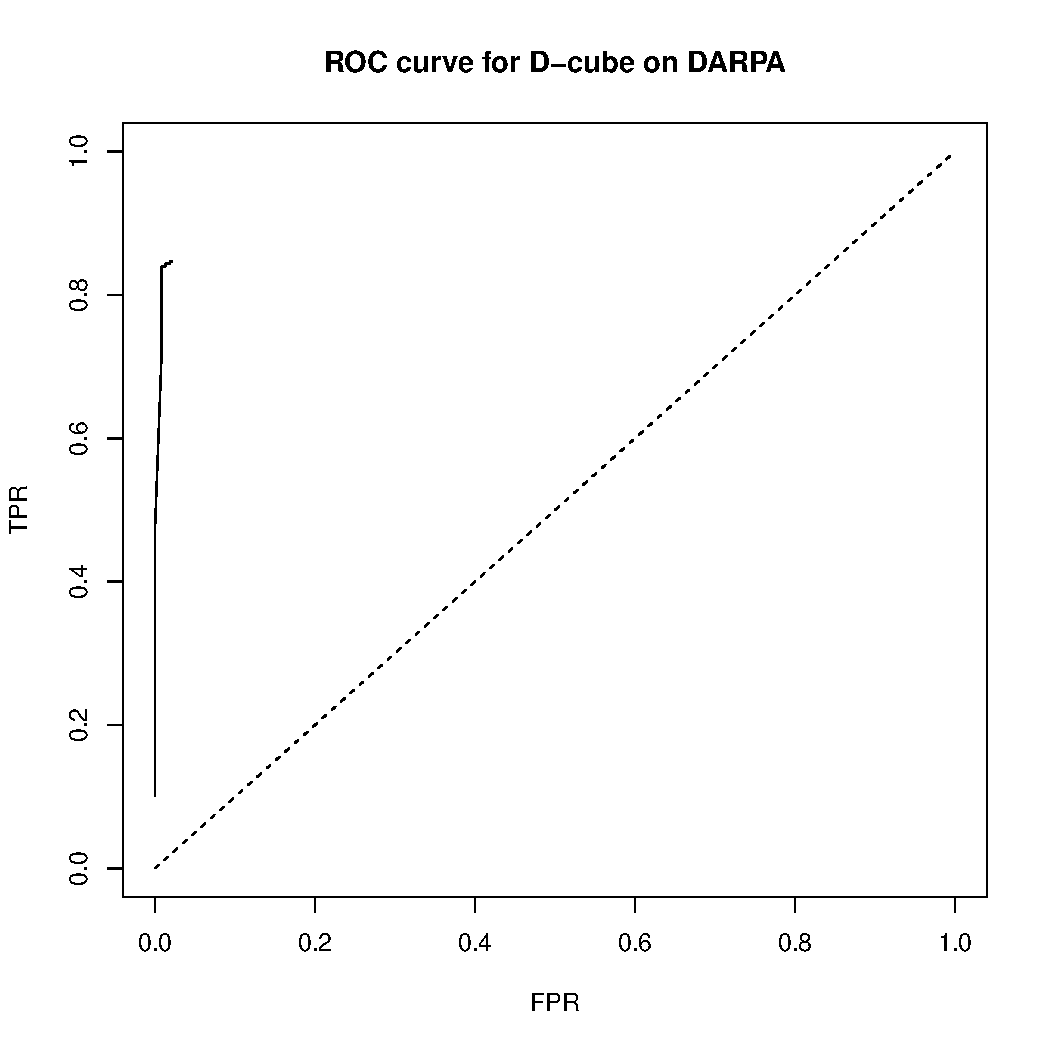
\includegraphics[width=.45\columnwidth]{plots/darpa_ROC.pdf} 
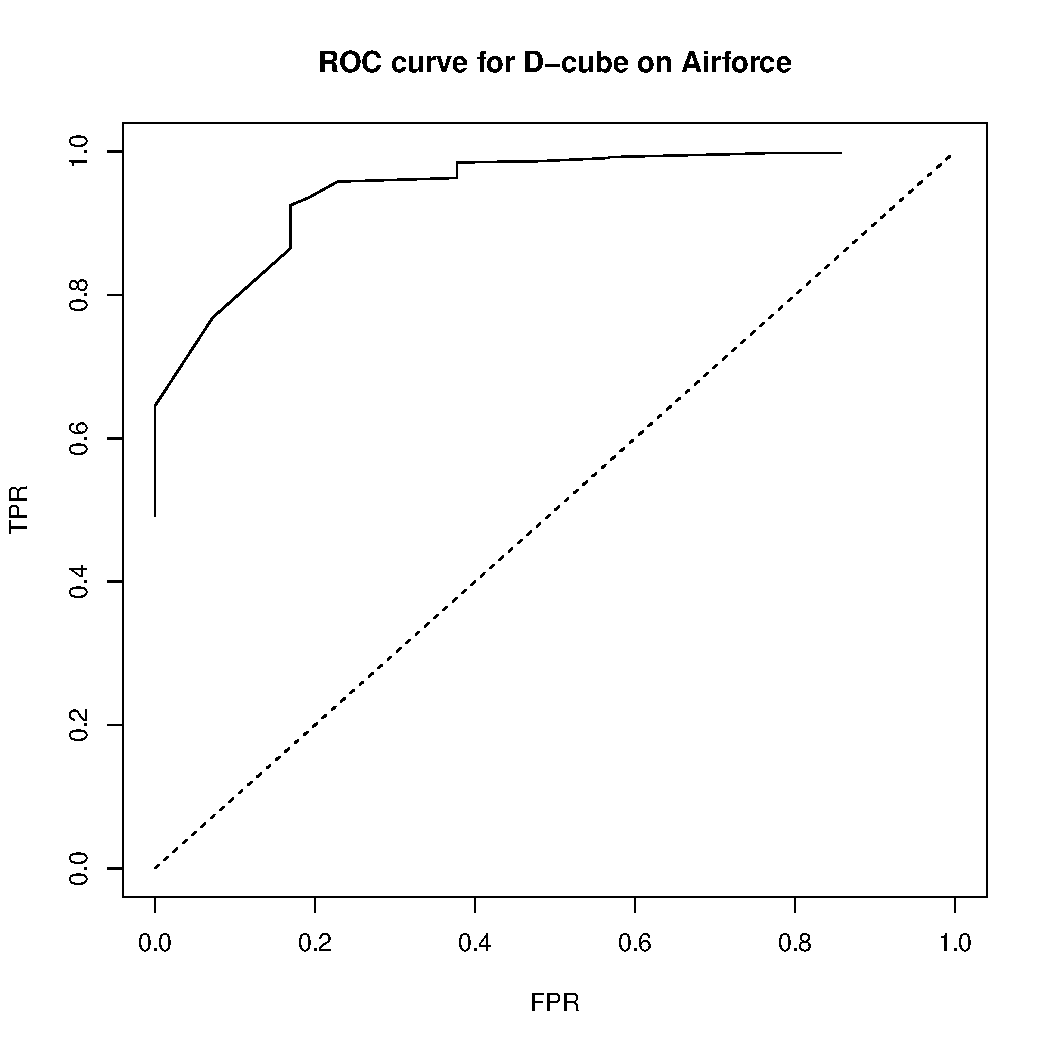
\includegraphics[width=.45\columnwidth]{plots/airforce_ROC.pdf} 
\caption{The ROC curve for $k = 1, \cdots, 20$ by applying the D-cube algorithm on the DARPA TCP Dump dataset (left) and Airforce TCP Dump dataset (right). }
\label{fig: roc}
\end{figure}


\subsection{Anomaly Detection in Real-world Data}
We also applied our implementation on the other three real-world datasets using maximum density policy for dimension selection. We used arithmetic density measure for Yelp and Amazon dataset, and geometric density measure for Wikipedia dataset. Table \ref{table: k5_3} summarizes the information for the first five blocks identified in each dataset. 

We show a basic breakdown of all the labeled users in the first 5 blocks detected from the Wikipedia dataset in Table \ref{tab: wiki}. As can be seen, the majority of these edits come from a few users, which means the algorithm did detect program driven, un-humanlike behavior.

A somewhat intriguing observation is that both Yelp and Amazon have abnormally large 5th blocks. The volume and mass of the fifth block is orders of magnitude greater than the first four blocks. This is directly observable by the size of the files that identified blocks are written to. In the amazon dataset case, the first four block files are at most 166KB, yet the fifth block file is as large as 1.5MB.  In Table \ref{tab: amazon}, we show the number of star distribution in each of the first five blocks detected in the Amazon dataset. Block 1, 3, and 4 are more likely to be suspicious behavior, while we are not too sure about block 2 and 5, since the star distribution doesn't suit our imagination of a typical rating spamming operation. Similarly we show the number of star distribution in Table \ref{tab: yelp}. The first four blocks seem to be spam-like behaviors, since they all contain ratings with the same number of stars. The fifth block, however, contains a lot of ratings from 1 star to 5 star. We are not entirely sure whether that's an anomaly in the dataset or some bug with our implementation.

\begin{table}[htbp]
\centering
\caption{Summary of the first 5 blocks on Yelp, Amazon, and Wiki dataset}
\label{table: k5_3}
\begin{tabular}{rrrrr}
\hline
Dataset                                                                                    & Order                  & Volume & Mass   & Density  \\ \hline
\multirow{5}{*}{Yelp}                                                                      & \multicolumn{1}{r|}{1} & 3600   & 3600   & 118.03   \\
                                                                                           & \multicolumn{1}{r|}{2} & 3025   & 3025   & 108.04   \\
                                                                                           & \multicolumn{1}{r|}{3} & 2500   & 2500   & 98.04    \\
                                                                                           & \multicolumn{1}{r|}{4} & 2025   & 2025   & 88.04    \\
                                                                                           & \multicolumn{1}{r|}{5} & 336.7B & 268K   & 84.83    \\ \hline
\multirow{5}{*}{Amazon}                                                                    & \multicolumn{1}{r|}{1} & 3600   & 3600   & 118.03   \\
                                                                                           & \multicolumn{1}{r|}{2} & 135K   & 7550   & 99.02    \\
                                                                                           & \multicolumn{1}{r|}{3} & 1600   & 1600   & 78.05    \\
                                                                                           & \multicolumn{1}{r|}{4} & 1225   & 1225   & 68.06    \\
                                                                                           & \multicolumn{1}{r|}{5} & 30B    & 77.7K  & 50.34    \\ \hline
\multirow{5}{*}{\begin{tabular}[c]{@{}r@{}}Wikipedia\\ (Geometric\\ Density)\end{tabular}} & \multicolumn{1}{r|}{1} & 32     & 7865   & 2477.32  \\
                                                                                           & \multicolumn{1}{r|}{2} & 6696   & 16508  & 875.84   \\
                                                                                           & \multicolumn{1}{r|}{3} & 5      & 557    & 325.74   \\
                                                                                           & \multicolumn{1}{r|}{4} & 10     & 110    & 51.06    \\
                                                                                           & \multicolumn{1}{r|}{5} & 1974   & 6491   & 517.44   \\ \hline
\end{tabular}
\end{table}

\begin{table}[htbp]
\centering
\caption{Users in the first 5 blocks identified from the Wikipedia dataset}
\label{tab: wiki}
\begin{tabular}{r|lll}
\hline
\multicolumn{1}{l|}{Order} & \multicolumn{3}{c}{Labeled User}                              \\ \hline
1                                &     &       Cyberbot II: 32          &                        \\
2                                & AvicBot: 444       & Cydebot Ops: 744 & Ops Monitor (WMF): 744 \\
3                                & &      Wilhelmina Will: 5             &                        \\
4                                &  &     DeltaQuad Bot: 10              &                        \\
5                                &  &   DeltaQuadBot: 1903               &                        \\ \hline
\end{tabular}
\end{table}


\begin{table}[htbp]
\centering
\caption{Number of stars distribution in the first 5 blocks identified in the Amazon dataset}
\label{tab: amazon}
\begin{tabular}{r|ll}
\hline
\multicolumn{1}{l|}{Order} & \multicolumn{2}{l}{Number of stars: count} \\ \hline
1                          &                      & 5 star: 3600         \\
2                          & 1 star: 4525         & 4 star: 3025         \\
3                          &                      & 3 star: 1600         \\
4                          &                      & 1 star: 1225         \\
5                          & 1 star: 7041         & 2 star: 5151         \\
\multicolumn{1}{l|}{}      & 3 star: 10059        & 4 star: 16670        \\
\multicolumn{1}{l|}{}      &                      & 5 star: 38773        \\ \hline
\end{tabular}
\end{table}

\begin{table}[htbp]
\centering
\caption{Number of stars distribution in the first 5 blocks identified in the Yelp dataset}
\label{tab: yelp}
\begin{tabular}{r|ll}
\hline
\multicolumn{1}{l|}{Order} & \multicolumn{2}{r}{Number of stars: count} \\ \hline
1                          &                       & 5 star: 3600        \\
2                          &                       & 1 star: 3025        \\
3                          &                       & 3 star: 2500        \\
4                          &                       & 5 star: 2025        \\
5                          & 1 star: 106631        & 2 star: 76464       \\
\multicolumn{1}{l|}{}      & 3 star: 53380         & 4 star: 9957        \\
\multicolumn{1}{l|}{}      &                       & 5 star: 22107       \\ \hline
\end{tabular}
\end{table}